\section{Neural network architecture}
\subsection{U-Net architecture}
The standard architecture for image segmentation tasks in the medical imaging field is the U-Net \cite{ronneberger2015u}.

Figure \ref{unet} shows the architecture of the U-Net. The left side is called the encoder, the right side the decoder.

The encoder part is a standard deep convolutional neural network, doing standard feature detection with continuously bigger features using convolutional layers.

The decoder part on the right side is used to actually generate the segmentation output. The max pooling in the encoder part made the processed image continuously smaller,
to detect bigger features. The decoder does the counterpart, it increases the image until is has (almost) the same size as the input image again. It not only uses
the smallest feature map produced by the last convolutional layer of the encoder, but also the feature maps of the last convolutional layer of every encoder block.
A block contains two convolutional layers and corresponding ReLU activation functions. The upscaling from one decoder block to the next (the green arrows in the diagram) are
implemented with standard image upscaling algorithms like bilinear upsampling.


https://github.com/milesial/Pytorch-UNet
https://github.com/usuyama/pytorch-unet

modifications: do not use deprectated functions

\begin{figure}[H]
\centering
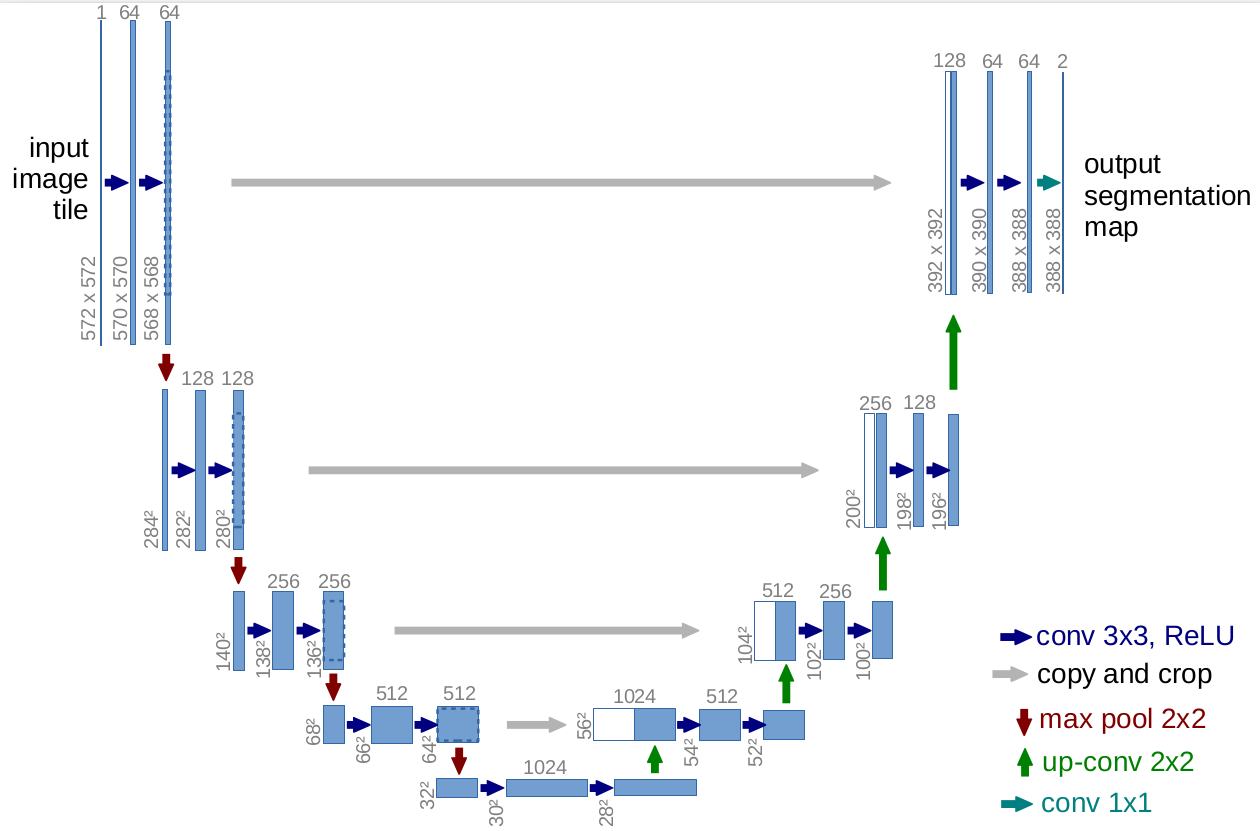
\includegraphics[width=14cm]{images/unet.png}
\caption{The U-Net architecture \cite{ronneberger2015u}.}
\label{unet}
\end{figure}
